\documentclass[12pt,a4paper]{article}
\usepackage[utf8]{inputenc}
\usepackage[russian]{babel}
\usepackage[OT1]{fontenc}
\usepackage{mathtools}
\usepackage{amsfonts}
\usepackage{amssymb}
\usepackage{enumitem}
\usepackage{alltt}
\usepackage{graphicx}
\usepackage{indentfirst}
\usepackage{caption}
\usepackage{float}
\usepackage{wrapfig}
\usepackage{physics}
\usepackage{multirow}
\usepackage{longtable}
\usepackage{amsmath,amsfonts,amssymb,amsthm,mathtools}
\usepackage{icomma}
\setlength{\parindent}{0.75cm}
\graphicspath{{pictures/}}
\DeclareGraphicsExtensions{.png}
\usepackage[left=15mm,right=15mm,top=2cm,bottom=2cm]{geometry}
\author{Глотов Алексей}
\begin{document}
\newpage
\begin{center}
\footnotesize{{ГОСУДАРСТВЕННОЕ АВТОНОМНОЕ ОБРАЗОВАТЕЛЬНОЕ УЧРЕЖДЕНИЕ}\break
{ВЫСШЕГО ОБРАЗОВАНИЯ}
\break
{\bf {МОСКОВСКИЙ ФИЗИКО-ТЕХНИЧЕСКИЙ ИНСТИТУТ}}
\break
\small{(НАЦИОНАЛЬНЫЙ ИССЛЕДОВАТЕЛЬСКИЙ УНИВЕРСИТЕТ)}}
\break
\hfill \break
\hfill \break
\begin{center}
\normalsize{Кафедра общей физики}
\end{center}
\hfill \break
\hfill \break
\hfill \break
\hfill \break

\begin{center}
\normalsize {Лабораторная работа 2.4.1}
\end{center}
\hfill \break\\
\large{\textbf{Определение теплоты испарения жидкости}}
\end{center}
\begin{flushleft}
\hfill \break
\hfill \break
\hfill \break
\hfill \break
\hfill \break
\hfill \break
\hfill \break
\hfill \break
\hfill \break
\hfill \break
\hangindent=9cm
\normalsize{Преподаватель:}\hfill
\normalsize{доцент Игуменов А.Ю.}\\
\hfill \break
\normalsize{Обучающийся:}\hfill
\normalsize{Глотов А.А} \\
\hfill \break
\end{flushleft}
\hfill \break
\hfill \break
\hfill \break
\hfill \break
\hfill \break
\hfill \break
\hfill \break
\hfill \break
\hfill \break
\hfill \break
\hfill \break

\begin{center}
Долгопрудный \break
 2022
\end{center}

\thispagestyle{empty}


\newpage
\section{Введение}

\subsection{Аннотация}

Данная работа посвящена изучению явления испарения жидкости при изменении температуры окружающей среды и давления насыщенных паров. Используются следующие методы: линеаризация и анализ графиков зависимости P(T). Значения T устанавливаем с помощью термостата, значения давления - при помощи гидростатического манометра (ртуть)

\textbf{Цель работы:}  \begin{enumerate}
	\item измерение давления насыщенного пара жидкости при разной температуре;
	\item вычисление по полученным данным теплоты испарения с помощью уравнения Клапейрона–Клаузиуса.
\end{enumerate}

\textbf{В работе используются:} термостат; герметический сосуд, заполненный исследуемой жидкостью; отсчетный микроскоп.

\subsection{Теоретические сведения}

Испарением называется переход вещества из жидкого в газообразное состояние. Оно происходит на свободной поверхности жидкости. При испарении с поверхности вылетают молекулы, образуя над ней пар. Для выхода из жидкости молекулы должны преодолеть силы молекулярного сцепления. Кроме того, при испарении совершается работа против внешнего давления $ P $. Не все молекулы жидкости способны совершить эту работу, а только те из них, которые обладают достаточной кинетической энергией. Поэтому переход части молекул в пар приводит к обеднению жидкости быстрыми молекулами, т.е. к ее охлаждению. Чтобы испарение проходило без изменения температуры, к жидкости нужно подводить тепло. Количество теплоты, необходимое для изотермического испарения одного моля жидкости при внешнем давлении, равном упругости ее насыщенных паров, называется молярной теплотой испарения (парообразования).

\subsection{Схема эксперимента}

Экспериментальный прибор B представляет собой емкость 12, заполненную водой. В нее погружен запаянный прибор 13 с исследуемой жидкостью 14. Перед заполнением исследуемой жидкости воздух из запаянного прибора был удален, так что над жидкостью находится только её насыщенный пар. Давление пара определяется по ртутному манометру 15, соединенному с емкостью 13. Численная величина давления измеряется по разности показаний отсчетного микроскопа 16, настраиваемого последовательно на нижний и верхний уровни столбика ртути манометра. Показания микроскопа снимаются по шкале 17.

\subsection{Методика измерений}

Теплоту парообразования жидкостей можно измерять непосредственно при помощи калориметра. Такой метод, однако, не позволяет получить точных результатов из-за неконтролируемых потерь тепла, которые трудно сделать малыми. В настоящей работе для определения теплоты испарения применен косвенный метод, основанный на формуле Клапейрона–Клаузиуса:

\begin{equation}\label{Kl-Kl}
\frac{dP}{dT}=\frac{L}{T\left(V_2-V_1\right)}.
\end{equation}

Здесь $ P $ -- давление насыщенного пара жидкости при температуре $ T $, $ T $ -- абсолютная температура жидкости и пара, $ L $ -- теплота испарения жидкости, $ V_2 $ -- объем пара, $ V_1 $ -- объем жидкости. Найдя из опыта $ dP/dT $, $ T $, $ V_2 $ и $ V_1 $, можно определить $ L $ путем расчета. Величины $ L $, $ V_2 $ и $ V_1 $ в формуле \eqref{Kl-Kl} должны относиться к одному и тому же количеству вещества; мы будем относить их к одному молю.

В нашем приборе измерения производятся при давлениях ниже атмосферного. В этом случае задача существенно упрощается.

При нашей точности опытов величиной $ V_1 $ в \eqref{Kl-Kl} можно пренебречь.

Обратимся теперь к $ V_2 $, которое в дальнейшем будем обозначать просто $ V $. Объем $ V $ связан с давлением и температурой уравнением Ван-дер-Ваальса:

\begin{equation}\label{VDV}
\left(P+\frac{a}{V^2}\right)\left(V-b\right)=RT.
\end{equation}

Из табличных данных следует, что $ b $ одного порядка с $ V_1 $. В уравнении Ван-дер-Ваальса величиной $ b $ следует пренебречь. Пренебрежение членом $ a/V^2 $ по сравнению с $ P $ вносит ошибку менее 3\%. При давлении ниже атмосферного ошибки становятся еще меньше. Таким образом, при давлениях ниже атмосферного уравнение Ван-дер-Ваальса для насыщенного пара мало отличается от уравнения Клапейрона. Положим поэтому

\begin{equation}\label{Volume}
V=\frac{RT}{P}.
\end{equation}

Подставляя \eqref{Volume} в \eqref{Kl-Kl}, пренебрегая $ V_1 $ и разрешая уравнение относительно $ L $, найдем

\begin{equation}\label{final}
L=\frac{RT^2}{P}\frac{dP}{dT}=-R\frac{d(\ln P)}{d(1/T)}.
\end{equation}

В нашем опыте температура жидкости измеряется термометром, давление пара определяется при помощи манометра, а производные $ dP/dT $ или $ d(\ln P)/d(1/T) $ находятся графически как угловой коэффициент касательной к кривой $ P(T) $ или соответственно к кривой, у которой по оси абсцисс отложено $ 1/T $, а по оси ординат $ \ln P $.

\subsection{Экспериментальная установка}

\begin{wrapfigure}{r}{6.5cm}
	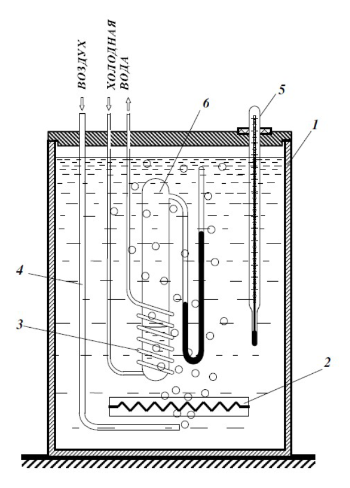
\includegraphics[width=6.5cm]{2.4.1_1}
	\caption{\textit{Схема первой установки}}
	\label{img1}
\end{wrapfigure}

Схема установки изображена на рисунке 1. Наполненный водой резервуар 1 играет роль термостата. Нагревание термостата производится спиралью 2, подогреваемой электрическим током. Для охлаждения воды в термостате через змеевик 3 пропускается водопроводная вода. Вода в термостате перемешивается воздухом, поступающим через трубку 4. Температура воды измеряется термометром 5. В термостат погружен запаянный прибор 6 с исследуемой жидкостью. Над ней находится насыщенный пар (перед заполнением прибора воздух из него был откачан). Давление насыщенного пара определяется по ртутному манометру, соединенному с исследуемым объемом. Отсчет показаний манометра производится при помощи микроскопа.

На рисунке \ref{img2} приведена более полная схема такой же установки, но с использованием современного термостата. Установка включает термостат A, экспериментальный прибор B и отсчетный микроскоп C.


Описание прибора указывает на второе важное преимущество предложенного косвенного метода измерения $ L $ перед прямым. При непосредственном измерении теплоты испарения опыты нужно производить при неизменном давлении, и прибор не может быть запаян. При этом невозможно обеспечить такую чистоту и неизменность экспериментальных условий, как при нашей постановке опыта.

Описываемый прибор обладает важным недостатком: термометр определяет температуру термостата, а не исследуемой жидкости (или ее пара). Эти температуры близки друг к другу лишь в том случае, если нагревание происходит достаточно медленно. Убедиться в том, что темп нагревания не является слишком быстрым, можно, сравнивая результаты, полученные при нагревании и при остывании прибора. Такое сравнение необходимо сделать. Для ориентировки укажем, что температуру воды в калориметре следует менять не быстрее, чем на 1 $ ^\circ C $ в течение 1–3 минут.

\begin{figure}[H]
\begin{center}
		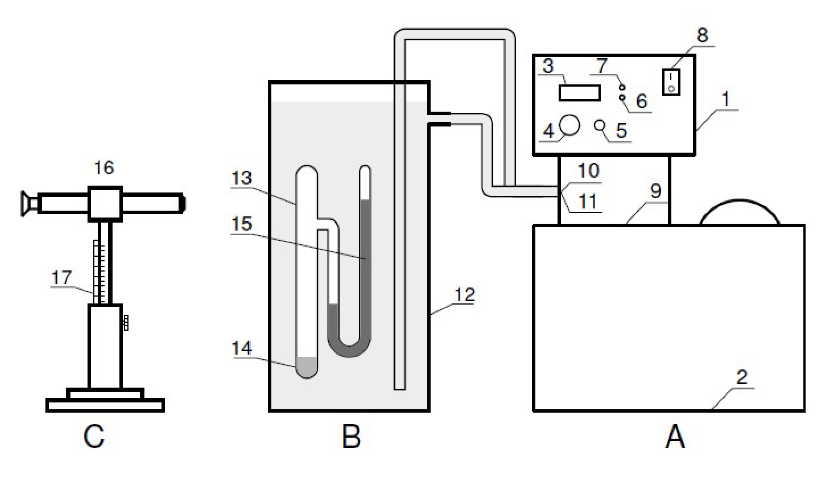
\includegraphics[width=15cm]{2.4.1_2}
\end{center}
	\caption{\textit{Схема второй установки}}
	\label{img2}
\end{figure}

\section{Результаты измерений и обработка данных}

\subsection{Проведение измерений}

Для определения теплоты парообразования воды измерим давление насыщенного пара при различных значениях температуры. Давление определяем при помощи ртутного манометра. При помощи штангенциркуля находим высоты $ h_1 $ и $ h_2 $ ртутных столбиков и по формуле  \begin{equation}\label{P}
\Delta P = \rho g (h_1 - h_2)
\end{equation}  находим давление насыщенного пара при определённой температуре. Результаты измерений заносим в таблицу \ref{tab:measures}.

При оценки погрешности измерения давления по формуле \eqref{P} следует использовать следующие соотношения:
\[ \sigma^2_{A\pm B} = \sigma^2_A+\sigma^2_B, \]
\[ \varepsilon^2_{A\cdot B} = \varepsilon^2_A+\varepsilon^2_B. \]

\begin{table}[H]
	\centering
	\begin{tabular}{|c|c|c|c|c|}
		\hline
		$ T $, К & $ h_1 $, мм & $ h_2 $, мм & $ \Delta P $, Па \\
		\hline
		293 & 96.30 & 81.9 & 1919.2 \\
		\hline
		294 & 96,80 & 81,90 & 1985,9 \\
		\hline 
		295 & 97,50 & 81,90 & 2079,2  \\
		\hline 
		296 & 98,00 & 81,90 & 2145,8  \\
		\hline 
		297 & 98,70 & 81,90 & 2239,1  \\
		\hline 
		298 & 99,50 & 81,90 & 2345,7 \\
		\hline
		299 & 100,20 & 81,90 & 2412,4 \\
		\hline
		300 & 101,30 & 81,90 & 2559,0 \\
		\hline
		301 & 102,00 & 81,90 & 2652,3 \\
		\hline
		302 & 102,70 & 81,90 & 2745,6 \\
		\hline
		303 & 103,80 & 81,90 & 2892,2 \\
		\hline
		304 & 104,90 & 81,90 & 3038,8 \\
		\hline
		305 & 105,70 & 81,90 & 3145,4 \\
		\hline
		306 & 106,80 & 81,90 & 3292,0 \\
		\hline
		307 & 107,90 & 81,90 & 3438,6 \\
		\hline
		308 & 109,20 & 81,90 & 3571,9 \\
		\hline
		309 & 110,50 & 81,90 & 3705,2 \\
		\hline
		310 & 111,30 & 81,90 & 3811,8 \\
		\hline
		311 & 112,50 & 81,90 & 3998,4 \\
		\hline
		312 & 113,60 & 81,90 & 4145,0 \\
		\hline
		313 & 114,50 & 81,90 & 4331,6 \\
		\hline
	\end{tabular}
	\caption{Измерение зависимости давления насыщенного пара от температуры жидкости}
	\label{tab:measures}
\end{table}

\subsection{Определение теплоты парообразования по графику $ P(T) $}

По данным из таблицы \ref{tab:measures} построим график зависимости давления насыщенного пара от температуры.

\begin{figure}[H]
\begin{center}
		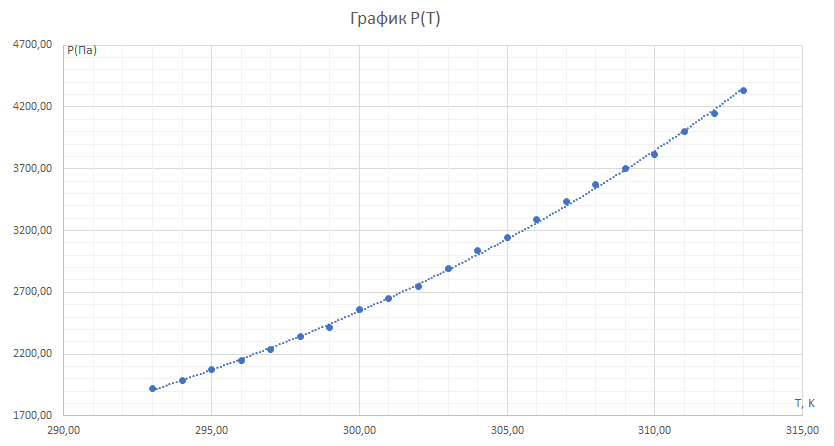
\includegraphics[width=15cm]{2.4.1_gr_1}
\end{center}
\end{figure}


Аппроксимируем методом наименьших квадратов полученные на этом участке температур зависимости функциями вида \[ P=ae^{bT}, \] где $ a $ и $ b $ -- неизвестные параметры. Используем следующие формулы:

\[ b = \frac{\langle \ln P \cdot T \rangle - \langle T \rangle \langle \ln P \rangle}{\langle T^2 \rangle - \langle T \rangle ^2},\]
\[ \ln a = \langle \ln P \rangle - b\langle T \rangle. \]

Случайные погрешности вычисления этих величин находим по следующим формулам:

\[ \sigma^\text{случ}_b = \sqrt{\frac{1}{N-2} \left(\frac{\left\langle\left(\ln P - \langle \ln P\right\rangle\right)^2 \rangle}{\left\langle\left(T - \langle T\right\rangle\right)^2 \rangle}\right)-b^2},\]
\[ \sigma^\text{случ}_{\ln a}=\sigma^\text{случ}_b\sqrt{\left\langle T^2 \right\rangle}. \]

\label{mnk}

Вкладом систематической погрешности в общую можно пренебречь в виду её малости по сравнению со случайной погрешностью определения коэффициентов. Поэтому будем считать, что \[ \sigma_b \approx \sigma^\text{случ}_b, \] \[ \sigma_{\ln a} \approx \sigma^\text{случ}_{\ln a}. \]

Полученные результаты заносим в таблицу \ref{tab:ab} и наносим зависимости на график.

\begin{table}[H]
	\centering
	\begin{tabular}{|c|c|c|c|}
		\hline
		$ a \cdot 10^{-3}$, Па & $ \sigma_a \cdot 10^{-3}$, Па & $ b \cdot 10^{-2} $, К$ ^{-1} $ & $ \sigma_b \cdot 10^{-2} $, К$ ^{-1} $ \\ \hline
		1.90 & 0,29 & 4,68 & 0,05 \\ \hline
	\end{tabular}
	\caption{Определение коэффициентов зависимости}
	\label{tab:ab}
\end{table}

Используя полученные результаты, можно получить формулу для производной давления по температуру: 
\begin{equation}\label{dpdt}
\frac{dP}{dT} = abe^{bT}.
\end{equation}
Подставляя \eqref{dpdt} в \eqref{final}, получаем:
\begin{equation}\label{newFinal}
L=\frac{RT^2ab}{P}e^{bT}.
\end{equation}

По полученным выше формулам вычисляем теплоту парообразования воды. Погрешность вычисления этой величины можно оценить по следующим формулам:
\[ \sigma_L = L\varepsilon_{\frac{dP}{dT}}, \]
\[ \sigma_{\frac{dP}{dT}} = \sqrt{\left(\frac{\partial\frac{dP}{dT}}{\partial a}\sigma_a\right)^2+\left(\frac{\partial\frac{dP}{dT}}{\partial b}\sigma_b\right)^2} \]

Полученные результаты заносим в таблицу \ref{tab:par}.

Полученные в этой части работы значения затем сравним со значениями, которые будут получены другим методом в следующей части.

\begin{table}[H]
	\centering
	\begin{tabular}{|c|c|c|}
	\hline
		$ T $, К & $ L $, $ \frac{\text{кДж}}{\text{моль}} $ & $ \sigma_L $, $ \frac{\text{кДж}}{\text{моль}} $ \\
		\hline
		293 & 30.0 & 4.7 \\ 
		\hline
		294 & 30.6 & 4.8 \\ 
		\hline 
		295 & 30.9 & 4.8 \\ 
		\hline 
		296 & 31.5 & 4.9 \\ 
		\hline 
		297 & 31.8 & 5.0 \\ 
		\hline 
		298 & 32.1 & 5.0 \\ 
		\hline 
		299 & 32.9 & 5.1 \\ 
		\hline 
		300 & 32.7 & 5.1 \\ 
		\hline 
		301 & 33.3 & 5.2 \\ 
		\hline 
		302 & 33.9 & 5.3 \\ 
		\hline
		303 & 34.0 & 5.3 \\ 
		\hline 
		304 & 34.1 & 5.3 \\ 
		\hline 
		305 & 34.8 & 5.4 \\ 
		\hline 
		306 & 35.0 & 5.5 \\ 
		\hline 
		307 & 35.4 & 5.5 \\ 
		\hline 
		308 & 35.9 & 5.6 \\ 
		\hline 
		309 & 36.5 & 5.7 \\ 
		\hline 
		310 & 37.5 & 5.9 \\ 
		\hline 
		311 & 37.7 & 5.9 \\ 
		\hline 
		312 & 38.3 & 6.0 \\ 
		\hline
		313 & 38.7 & 6.0 \\
		\hline 
	\end{tabular}
	\caption{Результаты вычисления теплоты парообразования}
	\label{tab:par}
\end{table}

Усредняя все наши значения L, получим, что

\[ L_ = \left(35.9 \pm 0,5\right) \text{ } \frac{\text{кДж}}{\text{моль}}, \]

\subsection{Определение теплоты парообразования по графику $ \ln P $ от $ 1 / T $}

Для построения графика преобразуем данные из таблицы \ref{tab:measures}. Преобразованные результаты измерений занесём в таблицу \ref{tab:ln}. Полученные значения наносим на график.

\begin{figure}[H]
\begin{center}
		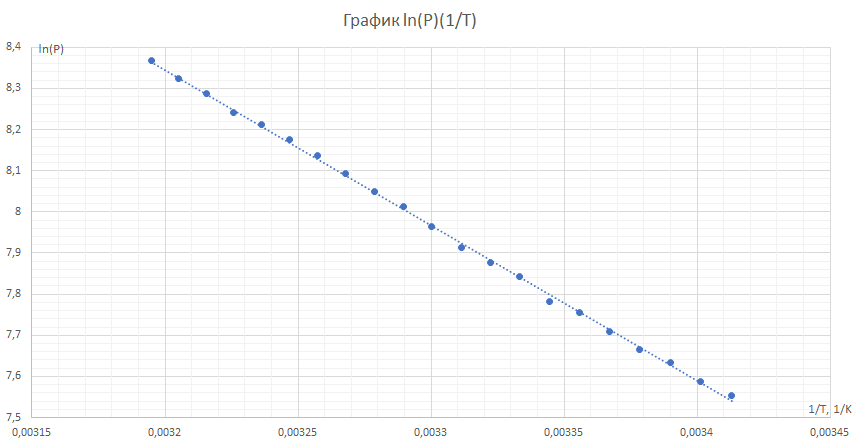
\includegraphics[width=15cm]{2.4.1_gr_2}
\end{center}
\end{figure}

\begin{table}[H]
	\centering
	\begin{tabular}{|c|c|}
		\hline
		$ T \cdot 10^{-3} $, К$ ^{-1} $ & $ \ln P $ \\
		\hline
		3,411 & 7.55 \\
		\hline
		3,401 & 7.59 \\
		\hline
		3,390 & 7.63 \\
		\hline
		3,378 & 7.67 \\
		\hline
		3,367 & 7.71 \\
		\hline
		3,356 & 7.76 \\
		\hline
		3,344 & 7.78 \\
		\hline
		3,333 & 7.84 \\
		\hline
		3,322 & 7.88 \\
		\hline
		3,311 & 7.91 \\
		\hline
		3,300 & 7.96 \\
		\hline
		3,289 & 8.01 \\
		\hline
		3,279 & 8.05 \\
		\hline
		3,268 & 8.09 \\
		\hline
		3,257 & 8.14 \\
		\hline
		3,247 & 8.18 \\
		\hline
		3,236 & 8.21 \\
		\hline
		3,226 & 8.24 \\
		\hline
		3,215 & 8.29 \\
		\hline
		3,205 & 8.32 \\
		\hline
		3,195 & 8.37 \\
		\hline
	\end{tabular}
	\caption{Зависимость $\ln P$ от $1/T$}
	\label{tab:ln}
\end{table}

С помощью формул, описанных в \ref{mnk}, вычислим значение и погрешность определения коэффициента $ \displaystyle \frac{d(\ln P)}{d(1/T)} $ с помощью метода наименьших квадратов. Таким образом, получаем

\[ \left(\frac{d(\ln P)}{d(1/T)}\right) = \left(-4410\pm48\right)\text{ К}, \]


По формуле \eqref{final} вычисляем теплоту парообразования. Получаем:

\[ L_ = \left(36,7 \pm 0,4\right) \text{ } \frac{\text{кДж}}{\text{моль}}, \]


Полученные значения будут сравнены с эталонными значениями и со значениями, полученными в предыдущей части работы, в п. \ref{res}.

\section{Обсуждение результатов и выводы}
\label{res}

В ходе выполнения работы:

\begin{itemize}
	\item была исследована зависимость давления насыщенных паров воды от давления жидкости;
	\item были вычислены теплоты парообразования воды для различных температур двумя разными способами.
\end{itemize}

Теплота парообразования, определенная с помощью графика зависимости $P(T)$, пересчитанная в необходимые размерности из ранее полученных значений:


\[ \boxed{L = \left(2,0 \pm 0,3\right) \text{ } \frac{\text{кДж}}{\text{кг}} \quad (\varepsilon = 15 \%),} \]


Также теплота парообразования была определена при помощи графика зависимости $ \ln P $ от $ 1/T $. По результатам этих измерений получили:

\[ \boxed{L = \left(2,04 \pm 0,02\right) \text{ } \frac{\text{МДж}}{\text{кг}} \quad (\varepsilon = 1,1 \%),} \]


Данные, полученные при помощи двух различных методов, вполне совпадают друг с другом.

Сравним полученные данные с табличными. Из табличных данных:

\[ L = 2,26 \text{ } \frac{\text{МДж}}{\text{кг}}. \]

Таким образом, полученные данные достаточно близки с табличными. В пределах погрешности с табличными данными совпадают результаты по точечного измерения теплоты парообразования. В тоже время, у этого метода высокая случайная погрешность вычисления.

При вычислении теплоты парообразования по графику зависимости $ \ln P $ от $ 1/T $ мы получаем среднее значение для всего исследуемого отрезка температур. Из-за этого у данного метода небольшая погрешность, т.к. происходит усреднение по множеству точек.





\end{document}